% Created 2011-02-22 Tue 10:01
\documentclass[11pt]{article}
\usepackage[utf8]{inputenc}
\usepackage[T1]{fontenc}
\usepackage{fixltx2e}
\usepackage{graphicx}
\usepackage{longtable}
\usepackage{float}
\usepackage{wrapfig}
\usepackage{soul}
\usepackage{textcomp}
\usepackage{hyperref}
\tolerance=1000
\usepackage{amsmath}
\usepackage{color}
\usepackage{stmaryrd}
\usepackage{listings}
\usepackage{attrib}
\providecommand{\alert}[1]{\textbf{#1}}
\begin{document}



\title{Active Documents with Org-mode}
\author{Eric Schulte and Dan Davison}
\date{22 February 2011}
\maketitle


\begin{abstract}

  Org-mode is a simple, plain text, markup language for hierarchical
  documents allowing intermingled data, code and prose.  An entire
  research project, including initial note taking, planning, task
  management, experimentation, analysis, and publication may take
  place within a single Org-mode document.  This article introduces
  Org-mode with an overview of syntax, a working \emph{reproducible}
  example of embedded data analysis, and a summary of the features
  that make Org-mode a particularly useful tool for the scientific
  researcher.

\end{abstract}

\section{Introduction}
\label{sec-1}

Org-mode is implemented as a part of the Emacs text editor
\cite{emacs}.  It was initially developed as a simple outlining tool
intended for note taking and brainstorming, and was later augmented
with task management tools---enabling notes to be transformed into
tasks with deadlines and priorities---and with syntax for the
inclusion of tables, data blocks, and active code blocks.  Users new
to Org-mode often start with its simple plain-text note taking system,
then move on to increasingly sophisticated features as their comfort
level permits.

Reproducible Research (RR) is the practice of publishing scientific
results along with the software environment and data required for
reproduction of all computational analyses presented in the
publication \cite{cise-rr}.  Reproducibility is essential to peer
reviewed research, however, scientific publications often lack the
information required for reviewers to reproduce the analysis described
in the work.

\begin{quote}
An article about computational science in a scientific publication
is \textbf{not} the scholarship itself, it is merely \textbf{advertising} of the
scholarship.  The actual scholarship is the complete software
development environment and complete set of instructions which
generated the figures.

\attrib{Donoho \cite{donoho}}
\end{quote}

Org-mode supports RR with syntax for including in-line data and code,
mechanisms for evaluating embedded code, and publishing functionality
that may be used to automate the computational analysis and generation
of figures.  This article will focus on the features of Org-mode
that support the practice of RR; information on other aspects of
Org-mode can be found in the manual \cite{org-manual} \footnote{\href{http://orgmode.org/manual/}{http://orgmode.org/manual/} } and the
community wiki \footnote{\href{http://orgmode.org/worg/}{http://orgmode.org/worg/} }.  The plain text Org-mode source of this
article is available for download \footnote{\href{https://github.com/eschulte/CiSE/raw/master/org-mode-active-doc.org}{https://github.com/eschulte/CiSE/raw/master/org-mode-active-doc.org} }; a user with the requisite
open-source software can
execute the source code examples, which analyze a dataset and create
graphics, and export the complete paper to one of several output
formats.
\section{Syntax}
\label{sec-2}
\subsection{Outlines}
\label{sec-2_1}

Org-mode documents are organized using a hierarchical outline.  The
outline can be folded and expanded, hiding or exposing as much of the
document as wanted.  Using this facility, even very
large documents can be comfortably navigated in a manner similar to
that of a file system.  Headlines are indicated by leading \texttt{*}'s as
shown below in the folded view of this article from within Org-mode.


\begin{verbatim}
* Introduction...
* Syntax...
** Outlines...
** Code and Data...
* Evaluation...
* Example Application...
** Download External Data...
** Parsing...
** Analysis...
** Display...
* Conclusion...
* COMMENT How to Export this Document...
* Footnotes...
\end{verbatim}

The \texttt{...}'s at the end of each line indicate that the content of the
heading is hidden from view.  Notice that the heading beginning with
the keyword \texttt{COMMENT} is not included in the exported document.
Org-mode uses many such keywords for associating information with
headlines.
\subsection{Code and Data}
\label{sec-2_2}

Using a simple `block' syntax, both code and data can be embedded in
Org-mode documents, as follows.

\begin{verbatim}
First a data block.
#+begin_example
  raw textual data
#+end_example

Second a code block.
#+begin_src sh
  echo "shell script code"
#+end_src
\end{verbatim}

Code and data blocks can be named, allowing their contents to be
referenced form elsewhere in the Org-mode file, as illustrated in the
following example where the shell script references the contents of
the data block.

\begin{verbatim}
First a data block.
#+results: raw-data
#+begin_example
  raw textual data
#+end_example

Second a code block.
#+begin_src sh :var text=raw-data
  echo $text|wc
#+end_src

#+results:
: 1       3      17
\end{verbatim}

Cross references between the code and data elements of an
Org-mode file turn Org-mode into a powerful multilingual programming
environment, in which data and code expressed in many different
programming languages may interact.
\section{Evaluation}
\label{sec-3}

Code and data references make possible strings of \emph{chained evaluation}.  Figure \ref{fig:chained-evaluation} shows the series of
actions which result when the \texttt{analyze} code block
(fig. \ref{fig:chained-evaluation}, 1) is evaluated
interactively or during export.

\begin{figure}[htb]
\centering
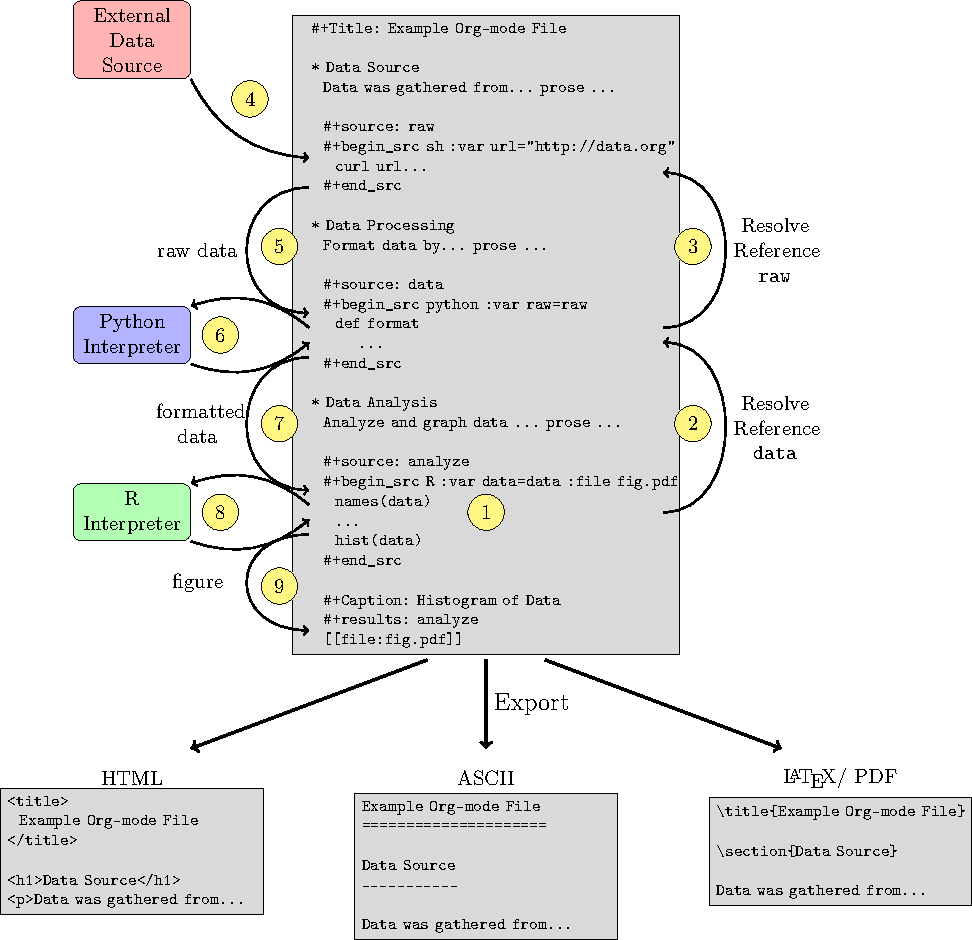
\includegraphics[width=\textwidth]{chained-evaluation.pdf}
\caption{\label{fig:chained-evaluation}Active Org-mode Document}
\end{figure}


\begin{enumerate}
\item The \texttt{analyze} code block is evaluated.  The \texttt{:var data=data} header
   argument causes Org-mode to evaluate the \texttt{data} reference.
\item To resolve this reference the \texttt{data} code block is located in the
   Org-mode file and is evaluated.
\item The \texttt{:var raw=raw} header argument causes Org-mode to resolve the
   \texttt{raw} reference.
\item The \texttt{raw} code block is evaluated, the \texttt{:var url="http://data.org"}
   header argument is evaluated as a literal value which is assigned
   to the \texttt{url} variable and passed to the shell script.

   The shell script then downloads data from the external url and
   makes these data available to Org-mode.
\item The results of the shell script are assigned to the \texttt{raw} variable,
   which is passed to the Python code in the body of the \texttt{data} code
   block.
\item This code is passed to an external Python interpreter which
   evaluates the Python code and returns its result to Org-mode.
\item The results of the \texttt{data} code block are then assigned to the
   \texttt{data} variable and passed to the R code in the body of the
   \texttt{analyze} code block.
\item This code is then passed to an external R interpreter, which
   generates a figure that is written to file specified in \texttt{:file fig.pdf}.
\item A reference to this figure is then passed from the \texttt{analyze} code
   block back to Org-mode, which inserts a link marked by double
   square brackets into the body of the Org-mode document.  On export
   to HTML, ASCII, \LaTeX{}, or another format supported by Org-mode,
   the linked figure will be embedded into the exported document.
\end{enumerate}
\section{Example Application}
\label{sec-4}

The application of Org-mode to RR is illustrated with an
analysis of baseball statistics.  The ordered nature of
baseball games makes them particularly amenable to statistical
analysis.  The performance of baseball players, and the course of
baseball games, are routinely captured in a small number of statistics
that are comparable across space and time.

In this example we analyze the correlation of several common offensive
statistics with the attendance at Major League Baseball (MLB) games in
the 2010 season.  We hypothesize what every baseball fan wants to
believe, that large crowds spur the home team to superior levels of
performance.  The offensive statistic that has the largest correlation
with high attendance is found and reported.
\subsection{Download External Data}
\label{sec-4_1}

This example will show correlation of home team offensive statistics
with attendance for the  \texttt{2010} MLB season.



This first code block, named \texttt{url}, translates the numerical season
shown above into the url for the \texttt{retrosheet.org} \footnote{The information used here was obtained free of charge from and
       is copyrighted by Retrosheet.  Interested parties may contact
       Retrosheet at ``www.retrosheet.org''. } website, a
website devoted to the collection and curation of major league
baseball statistics.



With the \texttt{raw-data} shell code block, the zip file of statistics located at
the specified url is downloaded and its contents are unpacked into a
local text file named \texttt{2010.csv}.  The \texttt{:cache yes} header argument
ensures that this code block is only run once and the data are not
downloaded again every time the results of the code block are referenced.



Next the \texttt{stat-headers} Python code block returns a list of the names of the
offensive statistics that will be tested for correlation with attendance.

\subsection{Parsing}
\label{sec-4_2}

The next two shell code blocks, \texttt{offensive-stats} and \texttt{attendance},
collect the offensive statistics and the attendance from the raw data
file produced by the \texttt{raw-data} code block.
\subsection{Analysis}
\label{sec-4_3}

The \texttt{analysis} code block uses the \texttt{R} statistical programming
language to calculate correlations between the outputs of the
\texttt{offensive-stats} and \texttt{attendance} code blocks, whose values are saved
into the \texttt{stats} and \texttt{attendance} variables respectively.



The most correlated column, namely  \texttt{intentional walks}, can
be mentioned in the text using an inline code block.  The Org-mode
syntax for an inline block can be seen below.


These results indicate that the fans' belief in the effect of large
crowds is shared by the visiting team, which chooses to walk a
dangerous home team hitter rather than take the chance that the large
crowd will spur him to a potentially damaging performance.
\subsection{Display}
\label{sec-4_4}

Using gnuplot we can plot the number of forced walks and the
attendance for the five games with the most forced walks (see Figure
\ref{fig:top-5}).

\begin{figure}[htb]
\centering
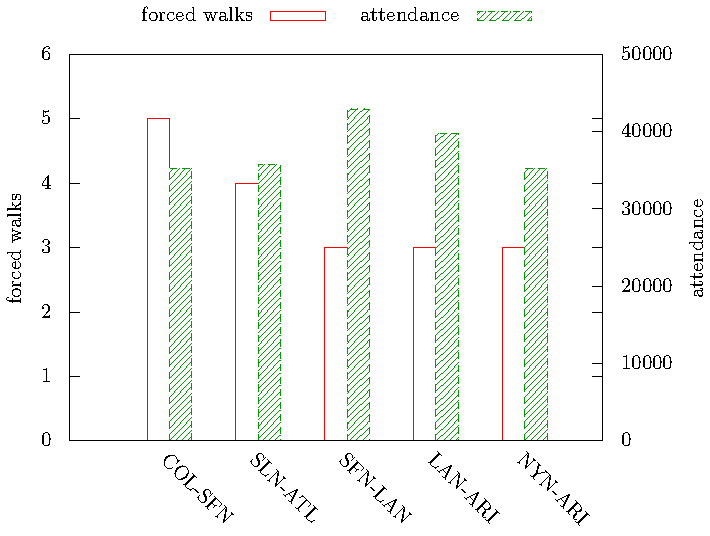
\includegraphics{plot.pdf}
\caption{\label{fig:top-5}Top 5 games by forced walks, with forced walks and attendance shown.}
\end{figure}

Commingling code and prose, as demonstrated in this example, makes it
possible for the author to collect all relevant information into a
single place.  This practice benefits the reader, who can reproduce
the calculations performed in the work, and also extend the analysis,
possibly within Org-mode itself.  For example, the reader of this
article can re-run the analysis for another season by simply changing
the value of the \texttt{season} code block above and re-exporting the file.
\section{Conclusion}
\label{sec-5}

There are a number of features of Org-mode that make it a good choice
for reproducible research; some of these are \emph{essential} for any RR
tool, and others alleviate common burdens of practicing RR.

Of the \emph{essential} properties, arguably the most important is that
as part of Emacs, the Org-mode copyright is owned by the Free Software
Foundation \cite{fsf}.  This ensures that Org-mode is now and will
always be free and open source software.  This is directly related to
two of the goals of RR.  First, Org-mode is available free of charge
to install by any user on any system ensuring access to the software
environment required for reproduction.  Second, the source code
specifying the inner workings of Org-mode is open to inspection,
ensuring that the mechanisms through which Org-mode generates
scientific results are open to review and verification.

In addition to its open source pedigree, Org-mode benefits in other
ways from its development as part of Emacs.  Emacs is one of the most
widely ported pieces of software in existence, with versions that run
on all major operating systems.  This ensures that Org-mode documents
can be incorporated into almost any computer working environment.
Emacs is also widely used by the scientific community for editing both
prose documents and source code.  By leveraging existing Emacs
editing support, Org-mode is able to offer its users a comfortable and
familiar editing environment for all types of content.  Finally, due
to Org-mode's implementation in the Emacs extension language, \emph{Emacs Lisp} \cite{elisp}, it is possible for users to customize the behavior
of Org-mode to their particular needs and to add support for arbitrary
new programming languages---Org-mode currently has support for over
thirty programming languages.

Org-mode addresses many common problems in the practice of RR.  Given
that a single Org-mode document can be used for every stage of a
research project from brain-storming, through software development and
experimentation, to publication, the author is largely relieved of the
burden of tracking resources required for reproduction of the work.
Such large amounts of information can result in extremely large
files, however the hierarchical folding of Org-mode documents enables
users to comfortably read and edit such files.  The files themselves are encoded in plain
text, which enhances their portability and makes them easy to integrate
well with version control systems, allowing for revision tracking and
collaboration \cite{cise-vc}.

Org-mode documents can run the gambit from simple collections of
plain-text notes, to complex laboratories housing data and analysis
mechanisms, to publishing desks with facilities for the display and
export of scientific results.  There is a friendly community of
Org-mode users and developers who communicate on the Org-mode
mailing list \footnote{\href{http://lists.gnu.org/mailman/listinfo/emacs-orgmode}{http://lists.gnu.org/mailman/listinfo/emacs-orgmode} }; through answering questions and helping each
other to master Org-mode's many features, this community helps to
solve one of the largest hurdles posed by any RR tool, namely learning
how to use it.

\bibliographystyle{plain}
\bibliography{babel}

\end{document}